% Schematic for the production-mix optimization example
% (CHEME-153-M2-ProductionMixOptimization-MWA-Graded-Codio-Activity.ipynb)
%
% Bipartite structure: 4 products (variables) consume 3 shared resources (constraints).
%   resource usage A[k,i] (rows = resources R1..R3, cols = products P1..P4):
%       R1: [2 1 1 2]   capacity b1 = 16
%       R2: [1 2 3 1]   capacity b2 = 20
%       R3: [1 1 1 3]   capacity b3 = 14
%   profit c = (6, 5, 4, 7);  budget sum(x) = tau = 8;  maximize c'x s.t. A x <= b.
%
% Build:  pdflatex production.tex
\documentclass[border=10pt]{standalone}
\usepackage{amsmath}
\usepackage{tikz}
\usetikzlibrary{arrows.meta, positioning, calc, decorations.pathreplacing, backgrounds}

\begin{document}
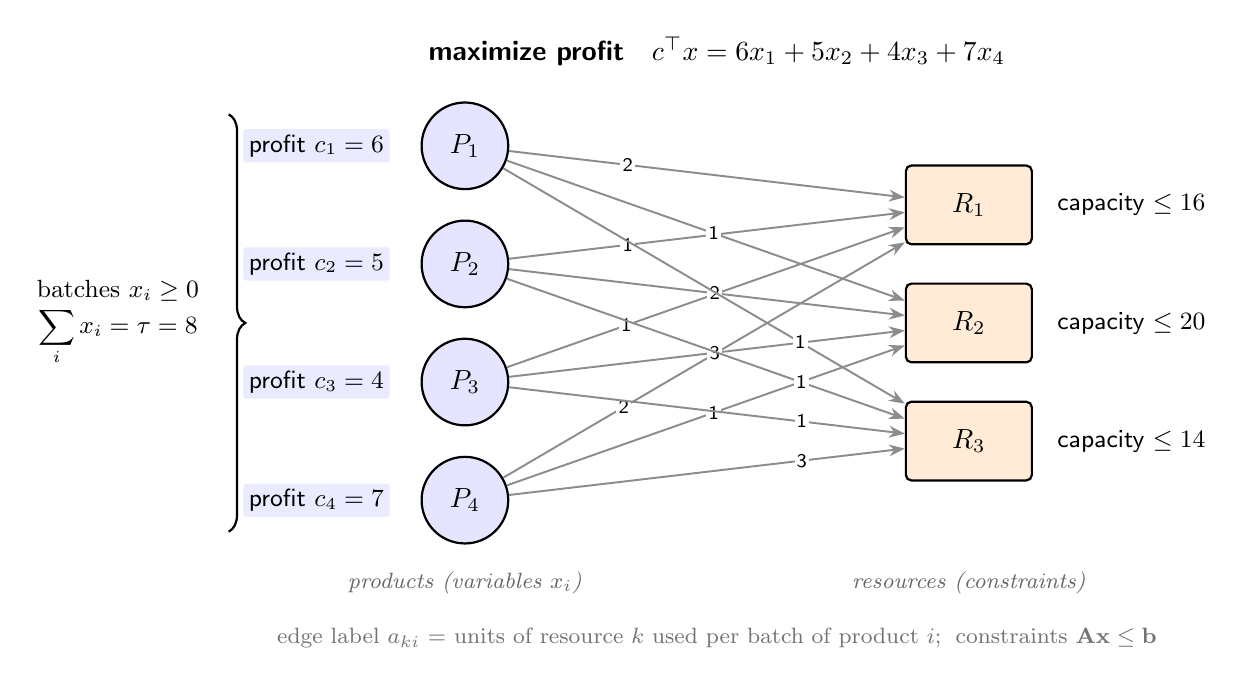
\begin{tikzpicture}[
    >={Stealth[length=2.4mm]},
    font=\sffamily,
    prod/.style = {circle, draw=black, line width=0.8pt, minimum size=11mm, inner sep=0pt, fill=blue!10},
    res/.style  = {rounded corners=2pt, draw=black, line width=0.8pt,
                   minimum width=16mm, minimum height=10mm, fill=orange!16},
    con/.style  = {-{Stealth[length=2.0mm]}, draw=black!45, line width=0.7pt},
    alab/.style = {font=\scriptsize\sffamily, fill=white, inner sep=0.8pt},
    ptag/.style = {font=\small\sffamily, anchor=east, fill=blue!8, rounded corners=1pt, inner sep=2pt},
    ctag/.style = {font=\small\sffamily, anchor=west}
  ]

  % --- products (left column) ---
  \node[prod] (P1) at (0,4.5) {$P_1$};
  \node[prod] (P2) at (0,3.0) {$P_2$};
  \node[prod] (P3) at (0,1.5) {$P_3$};
  \node[prod] (P4) at (0,0.0) {$P_4$};

  % --- resources (right column) ---
  \node[res] (R1) at (6.4,3.75) {$R_1$};
  \node[res] (R2) at (6.4,2.25) {$R_2$};
  \node[res] (R3) at (6.4,0.75) {$R_3$};

  % --- consumption edges  P_i --a_{ki}--> R_k  (labels staggered by resource) ---
  \draw[con] (P1) -- node[alab,pos=0.30]{2} (R1);
  \draw[con] (P2) -- node[alab,pos=0.30]{1} (R1);
  \draw[con] (P3) -- node[alab,pos=0.30]{1} (R1);
  \draw[con] (P4) -- node[alab,pos=0.30]{2} (R1);

  \draw[con] (P1) -- node[alab,pos=0.52]{1} (R2);
  \draw[con] (P2) -- node[alab,pos=0.52]{2} (R2);
  \draw[con] (P3) -- node[alab,pos=0.52]{3} (R2);
  \draw[con] (P4) -- node[alab,pos=0.52]{1} (R2);

  \draw[con] (P1) -- node[alab,pos=0.74]{1} (R3);
  \draw[con] (P2) -- node[alab,pos=0.74]{1} (R3);
  \draw[con] (P3) -- node[alab,pos=0.74]{1} (R3);
  \draw[con] (P4) -- node[alab,pos=0.74]{3} (R3);

  % --- profit tags (left of each product) ---
  \node[ptag] at (-0.95,4.5) {profit $c_1=6$};
  \node[ptag] at (-0.95,3.0) {profit $c_2=5$};
  \node[ptag] at (-0.95,1.5) {profit $c_3=4$};
  \node[ptag] at (-0.95,0.0) {profit $c_4=7$};

  % --- capacity tags (right of each resource) ---
  \node[ctag] at (7.4,3.75) {capacity $\le 16$};
  \node[ctag] at (7.4,2.25) {capacity $\le 20$};
  \node[ctag] at (7.4,0.75) {capacity $\le 14$};

  % --- budget brace (far left) ---
  \draw[decorate, decoration={brace, amplitude=6pt}, line width=0.8pt]
       (-3.0,4.9) -- (-3.0,-0.4)
       node[midway, left=7pt, align=center, font=\small]
       {batches $x_i \ge 0$\\[2pt] $\displaystyle\sum_{i} x_i=\tau=8$};

  % --- objective (top) ---
  \node[align=center, font=\sffamily] at (3.2,5.7)
       {\textbf{maximize profit}\quad $c^{\top}x = 6x_1+5x_2+4x_3+7x_4$};

  % --- column captions + edge-label key (bottom) ---
  \node[font=\footnotesize\itshape, black!60] at (0,-1.05) {products (variables $x_i$)};
  \node[font=\footnotesize\itshape, black!60] at (6.4,-1.05) {resources (constraints)};
  \node[font=\footnotesize, black!55, align=center] at (3.2,-1.75)
       {edge label $a_{ki}$ = units of resource $k$ used per batch of product $i$;\;
        constraints $\mathbf{A}\mathbf{x}\le\mathbf{b}$};

\end{tikzpicture}
\end{document}
